\begin{figure}
	\centering
%	\begin{minipage}[.3\textwidth]
		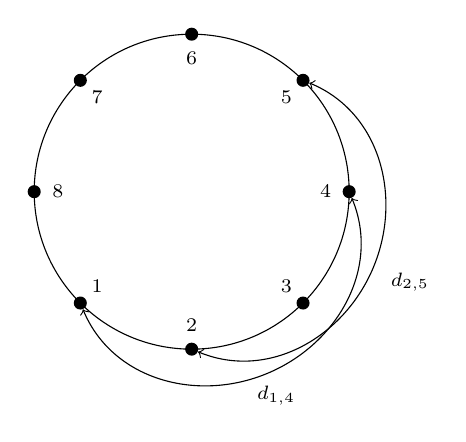
\begin{tikzpicture}[font=\scriptsize, node/.style={circle,thick,draw},scale=1, transform shape]
			% equidistant points and arc
			\foreach \x [count=\p] in {0,...,7} {
				\node[shape=circle,fill=black, scale=0.5] (\p) at (\x*45-135:2) {};
			};
			\foreach \x [count=\p] in {0,...,7} {
				\draw (225 + \x*45:1.7) node {\p};
%				\draw (-30-\x*60:2.4) node {$\bar{\p}$};
			}; 
			\draw (4) arc (0:360:2);
			\node (a) at (-22.5:3) {$d_{2, 5}$};
			\draw[<->] (2)  to [out=-22.5,in=-112.5] (-22.5:2.5) to [out=67.5,in=-22.5](5);
			\node (b) at (-67.5:2.8) {$d_{1, 4}$};
			\draw[<->] (1)  to [out=-67.5,in=-157.5] (-67.5:2.5) to [out=22.5,in=-67.5] (4);
			%		\draw[dashed] (1) -- (3) -- (5) -- (1);
			% axes
			%		\draw [dotted, gray] (-2.6,0) -- (2.6,0);
			%		\draw [dotted, gray] (0,-2.15) -- (0,2.15);
		\end{tikzpicture}
%	\end{minipage}
	\caption{Ring, demands, cuts and more }
	\label{fig:cut-example}
\end{figure}